% Permission is granted to copy, distribute and/or modify this document
% under the terms of the GNU Free Documentation License, Version 1.2
% or any later version published by the Free Software Foundation;
% with no Invariant Sections, no Front-Cover Texts, and no Back-Cover
% Texts.  A copy of the license is included in the section entitled "GNU
% Free Documentation License".
% Copyright 2016 EDF
%

%%%%%%%%%%%%%%%%%%%%%%%%%%%%%%%%%%%%%%%%%%%%%%%%%%%%%%%%%%%%%%%%%%%%%%%%%%%%%%%%%%%%%%%%%%
\section{Use cases}

\subsection{ANOVA table}

R listing
\begin{lstlisting}[style=RStyle]
# Output variables : weight of the plants
ctl <- c(4.17 ,5.58 ,5.18 ,6.11 ,4.50 ,4.61 ,5.17 ,4.53 , 5.33 ,5.14)
trt <- c(4.81 ,4.17 ,4.41 ,3.59 ,5.87 ,3.83 ,6.03 ,4.89 , 4.32 ,4.69)

# Input variables :
# - group " Ctl " : control group ( plant with standard conditions )
# - group " Trt " : Treatment group ( plant with nutritionally enriched environment )

group <- gl( 2, 10, 20, labels = c("Ctl","Trt"))
weight <- c(ctl,trt)

lm.D9 <- lm(weight ~ group)
summary(lm.D9)

### SAVE DATA
DATA = data.frame(cbind(ctl,trt))
names(DATA) = c("ctl","trt")
write.csv(DATA, file="DATA.csv",row.names=FALSE)
\end{lstlisting}

Output
\begin{lstlisting}[style=output]
Call:
lm(formula = weight ~ group)

Residuals:
    Min      1Q  Median      3Q     Max
-1.0710 -0.4938  0.0685  0.2462  1.3690

Coefficients:
            Estimate Std. Error t value Pr(>|t|)
(Intercept)   5.0320     0.2202  22.850 9.55e-15 ***
groupTrt     -0.3710     0.3114  -1.191    0.249
---
Signif. codes:  0 '***' 0.001 '**' 0.01 '*' 0.05 '.' 0.1 ' ' 1

Residual standard error: 0.6964 on 18 degrees of freedom
Multiple R-squared:  0.07308,   Adjusted R-squared:  0.02158
F-statistic: 1.419 on 1 and 18 DF,  p-value: 0.249
\end{lstlisting}

\newpage
Equivalent listing in python
\begin{lstlisting}[style=pythonStyle]
import openturns as ot

Sample = ot.NumericalSample.ImportFromTextFile("DATA.csv", ",")
ctl = Sample[:,0]
trt = Sample[:,1]

inputSample = ot.NumericalSample(ctl.getSize(), [0])
inputSample.add(ot.NumericalSample(trt.getSize(), [1]))
inputSample.setDescription(["Trt"])

outputSample = ctl
outputSample.add(trt)
outputSample.setDescription(["weight"])

algo = ot.LinearModelAlgorithm(inputSample, outputSample)
result = algo.getResult()
analysis = ot.LinearModelAnalysis(result)
print(analysis)
\end{lstlisting}

Output python
\begin{lstlisting}[style=output]
 Call:
Basis( [[Trt]->[1],[Trt]->[Trt]] )

 Coefficients:
             | Estimate    | Std Error   | t value     | Pr(>|t|)    | 
----------------------------------------------------------------------
[Trt]->[1]   | 5.032       | 0.220218    | 22.8501     | 9.54713e-15 | 
[Trt]->[Trt] | -0.371      | 0.311435    | -1.19126    | 0.249023    | 
----------------------------------------------------------------------

 Residual standard error: 0.69639 on 18 degrees of freedom 
 F-statistic: 1.4191 ,  p-value: 0.24822
----------------------------------
Multiple R-squared   | 0.0730776 | 
Adjusted R-squared   | 0.0215819 | 
----------------------------------

---------------------------------
Normality test       | p-value  | 
---------------------------------
Anderson-Darling     | 0.316615 | 
Chi-Squared          | 0.433749 | 
Kolmogorov-Smirnov   | 0.870208 | 
---------------------------------
\end{lstlisting}

\newpage
\subsection{Graphical diagnostics}

R listing
\begin{lstlisting}[style=RStyle,basicstyle=\footnotesize]
require(stats)
require(graphics)
## Analysis of the life-cycle savings data
## given in Belsley, Kuh and Welsch.

LifeCycleSavings <- read.table('LifeCycleSavings.csv', header=TRUE, sep=",")

lm.model1 <- lm(sr ~ pop15 + pop75 + dpi + ddpi , data=LifeCycleSavings)
plot(lm.model1 , which =1:6)

lm.model2 <- lm(sr^4 ~ pop75 + dpi , data=LifeCycleSavings)
plot(lm.model2 , which =1:6)
\end{lstlisting}

Equivalent listing in python
\begin{lstlisting}[style=pythonStyle,basicstyle=\footnotesize]
from openturns.viewer import View
import openturns as ot
import pandas as pd

# First column in this CSV file is country name, use
# pandas to easily filter it out.
data = pd.read_csv("LifeCycleSavings.csv", index_col=0)

Sample = ot.NumericalSample(data.values)
Sample.setName("LifeCycleSavings")
Sample.setDescription(["sr","pop15","pop75","dpi","ddpi"])

sr    = Sample[:,0]
pop15 = Sample[:,1]
pop75 = Sample[:,2]
dpi   = Sample[:,3]
ddpi  = Sample[:,4]

# model1
outputSample = Sample[:,0]
inputSample = Sample[:,1:5]

algo1 = ot.LinearModelAlgorithm(inputSample, outputSample)
result1 = algo1.getResult()
analysis1 = ot.LinearModelAnalysis(algo1.getResult())

for plot in ["drawResidualsVsFitted", "drawScaleLocation", "drawQQplot", "drawCookDistance", "drawResidualsVsLeverages", "drawCookVsLeverages"]:
    graph = getattr(analysis1, plot)()
    graph.draw("model1-"+plot, 640, 480)

# plot of residuals versus fitted values
graph = analysis1.drawResidualsVsFitted()
View(graph)

# scale-location plot of sqrt(|residuals|) versus fitted values
graph = analysis1.drawScaleLocation()
View(graph)

# Normal quantiles-quantiles plot of standardized residuals
graph = analysis1.drawQQplot()
View(graph)

# plot of Cook's distances versus row labels
graph = analysis1.drawCookDistance()
View(graph)

# plot of residuals versus leverages that adds bands corresponding to Cook's distances of 0.5 and 1
graph = analysis1.drawResidualsVsLeverages()
View(graph)

# plot of Cook's distances versus leverage/(1-leverage)
graph = analysis1.drawCookVsLeverages()
View(graph)

# model2
f = ot.NumericalMathFunction('x','x^4','y')
outputSample = f(sr)
inputSample = pop75
inputSample.stack(dpi)

algo2 = ot.LinearModelAlgorithm(inputSample, outputSample)
result2 = algo2.getResult()
analysis2 = ot.LinearModelAnalysis(algo2.getResult())

for plot in ["drawResidualsVsFitted", "drawScaleLocation", "drawQQplot", "drawCookDistance", "drawResidualsVsLeverages", "drawCookVsLeverages"]:
    graph = getattr(analysis2, plot)()
    graph.draw("model2-"+plot, 640, 480)

# plot of residuals versus fitted values
graph = analysis2.drawResidualsVsFitted()
View(graph)

# scale-location plot of sqrt(|residuals|) versus fitted values
graph = analysis2.drawScaleLocation()
View(graph)

# Normal quantiles-quantiles plot of standardized residuals
graph = analysis2.drawQQplot()
View(graph)

# plot of Cook's distances versus row labels
graph = analysis2.drawCookDistance()
View(graph)

# plot of residuals versus leverages that adds bands corresponding to Cook's distances of 0.5 and 1
graph = analysis2.drawResidualsVsLeverages()
View(graph)

# plot of Cook's distances versus leverage/(1-leverage)
graph = analysis2.drawCookVsLeverages()
View(graph)

\end{lstlisting}

\begin{figure}[p]
  \begin{center}
    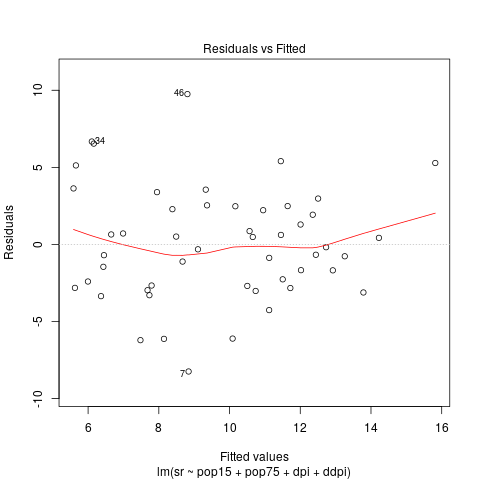
\includegraphics[scale=0.48]{imgR/plot11.png} \hspace*{2cm} 
	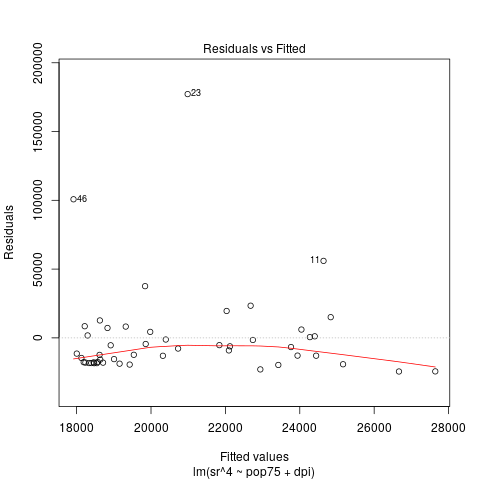
\includegraphics[scale=0.48]{imgR/plot21.png} \\
    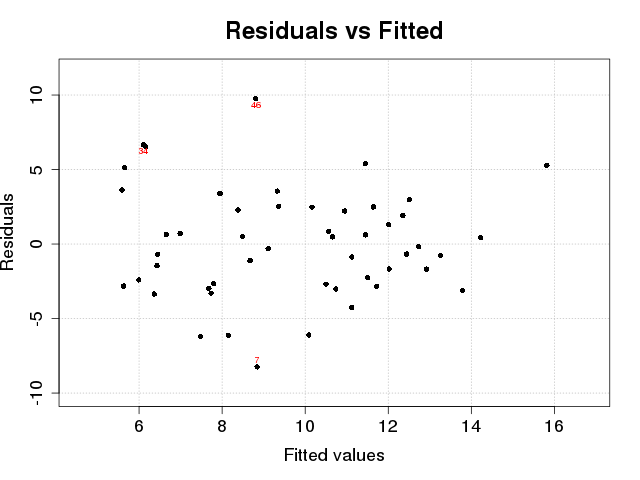
\includegraphics[scale=0.4]{imgOT/model1-drawResidualsVsFitted.png}\hspace*{1cm}
	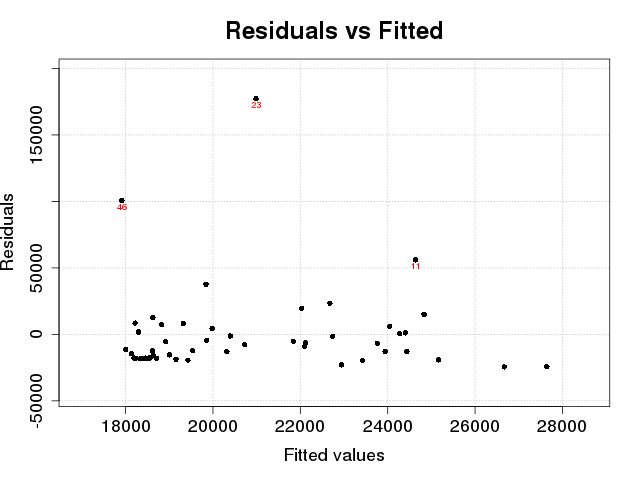
\includegraphics[scale=0.4]{imgOT/model2-drawResidualsVsFitted.png}\\
  \end{center}
  \caption{Draw residuals versus fitted values : \newline
  (Upper left: \textbf{\color{black}{model1: R output}}) (Upper right: \textbf{\color{black}{model2: R output}}) \newline
  (Lower left: \textbf{\color{blue}{model1: python output}})  (Lower right: \textbf{\color{blue}{model2: python output}}) }
\end{figure}

\begin{figure}[p]
  \begin{center}
    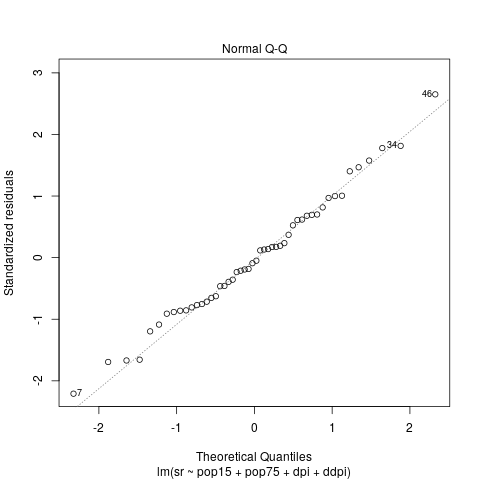
\includegraphics[scale=0.48]{imgR/plot12.png} \hspace*{2cm}
	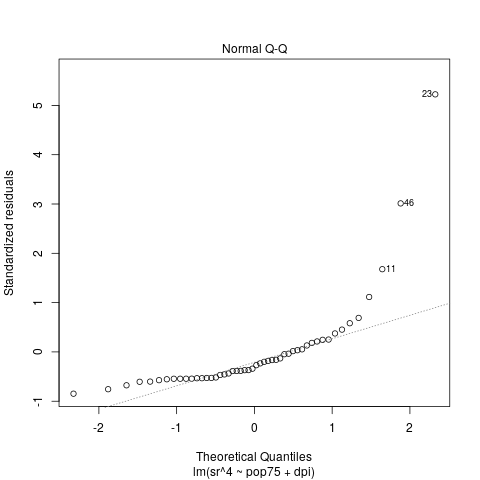
\includegraphics[scale=0.48]{imgR/plot22.png} \\
    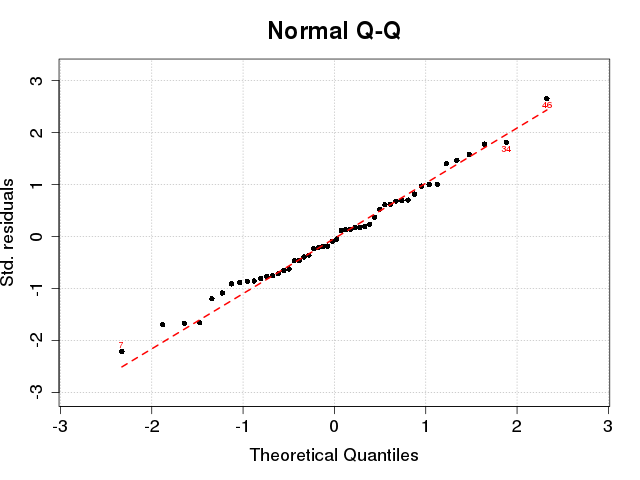
\includegraphics[scale=0.4]{imgOT/model1-drawQQplot.png}\hspace*{1cm}
	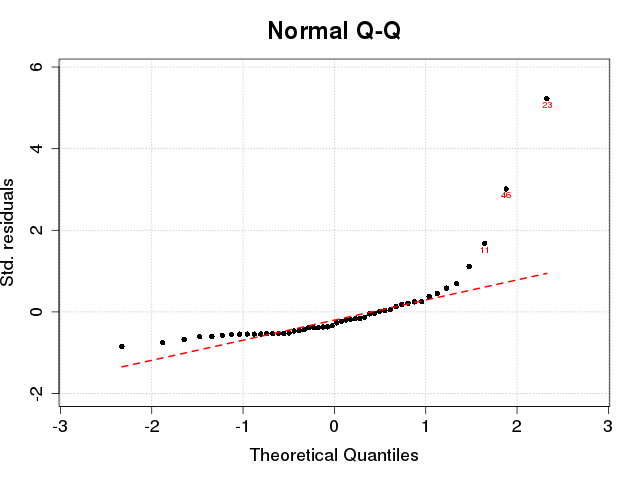
\includegraphics[scale=0.4]{imgOT/model2-drawQQplot.png}\\
  \end{center}
  \caption{Draw a Normal quantiles-quantiles plot of standardized residuals : \newline
  (Upper left: \textbf{\color{black}{model1: R output}}) (Upper right: \textbf{\color{black}{model2: R output}}) \newline
  (Lower left: \textbf{\color{blue}{model1: python output}})  (Lower right: \textbf{\color{blue}{model2: python output}}) }
\end{figure}

\begin{figure}[p]
  \begin{center}
    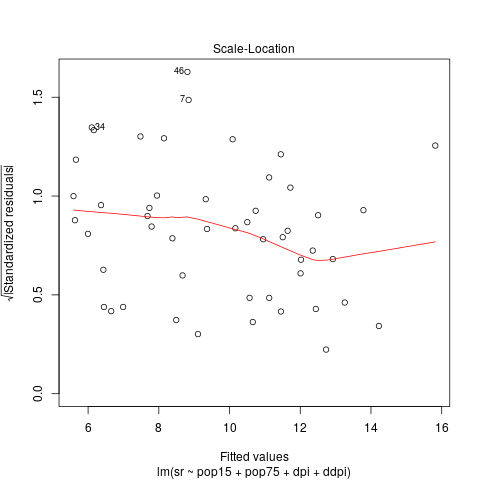
\includegraphics[scale=0.48]{imgR/plot13.png} \hspace*{2cm}
	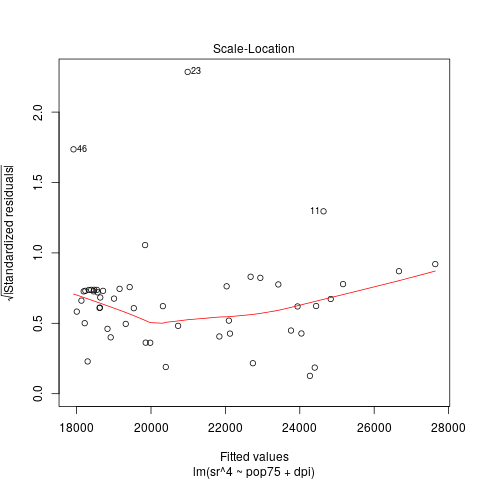
\includegraphics[scale=0.48]{imgR/plot23.png} \\
    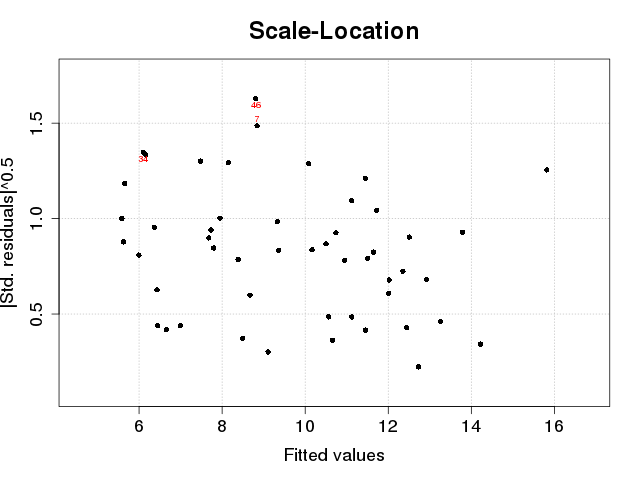
\includegraphics[scale=0.4]{imgOT/model1-drawScaleLocation.png}\hspace*{1cm}
	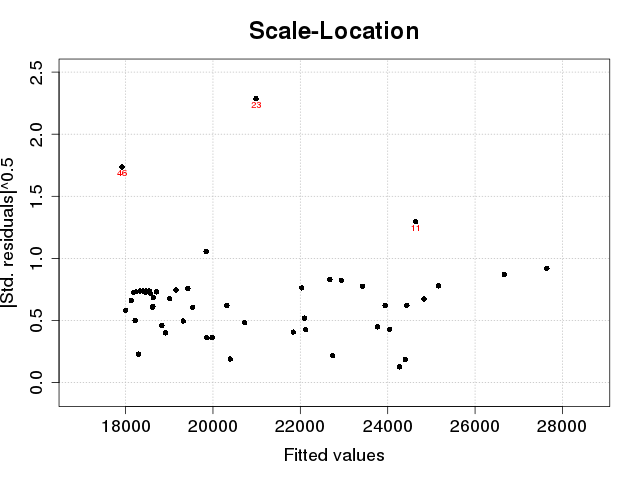
\includegraphics[scale=0.4]{imgOT/model2-drawScaleLocation.png}\\
  \end{center}
  \caption{Draw a Scale-Location plot of $\sqrt{\| \,\text{residuals}\,\|}$ versus fitted values :\newline
  (Upper left: \textbf{\color{black}{model1: R output}}) (Upper right: \textbf{\color{black}{model2: R output}}) \newline
  (Lower left: \textbf{\color{blue}{model1: python output}})  (Lower right: \textbf{\color{blue}{model2: python output}}) }
\end{figure}

\begin{figure}[p]
  \begin{center}
    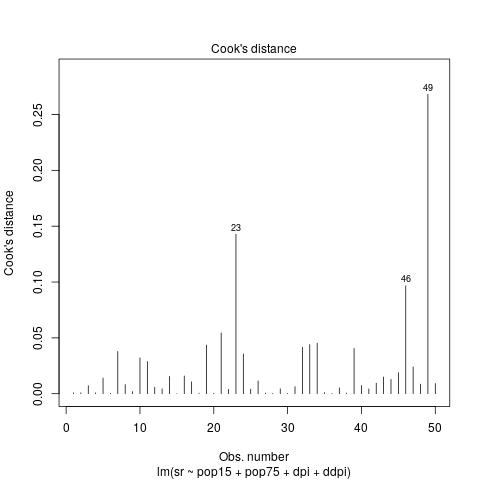
\includegraphics[scale=0.48]{imgR/plot14.png} \hspace*{2cm}
	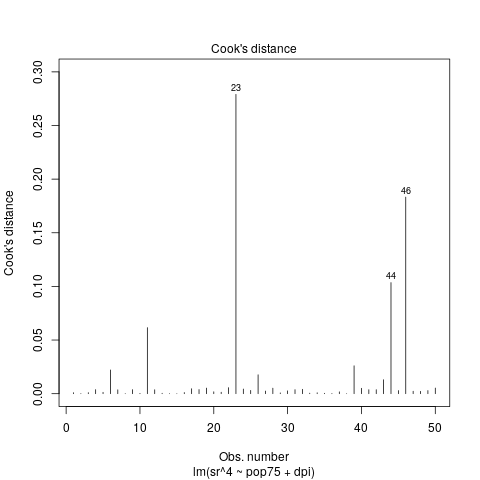
\includegraphics[scale=0.48]{imgR/plot24.png} \\
    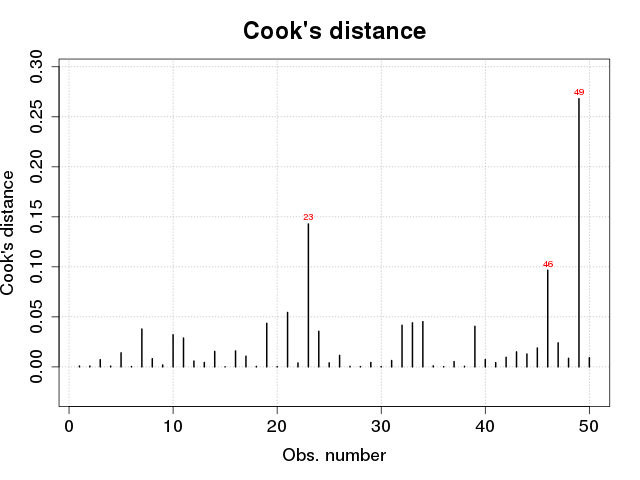
\includegraphics[scale=0.4]{imgOT/model1-drawCookDistance.png}\hspace*{1cm}
	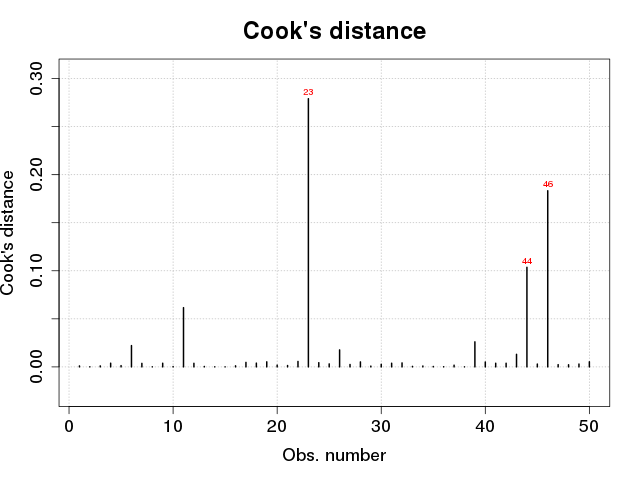
\includegraphics[scale=0.4]{imgOT/model2-drawCookDistance.png}\\
  \end{center}
  \caption{Draw Cook's distances versus row labels  :\newline
  (Upper left: \textbf{\color{black}{model1: R output}}) (Upper right: \textbf{\color{black}{model2: R output}}) \newline
  (Lower left: \textbf{\color{blue}{model1: python output}})  (Lower right: \textbf{\color{blue}{model2: python output}}) }
\end{figure}

\begin{figure}[p]
  \begin{center}
    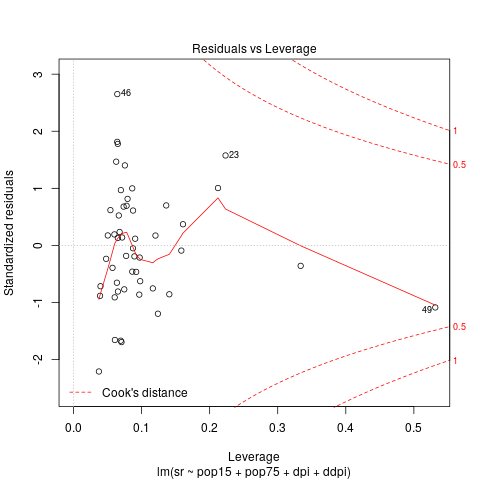
\includegraphics[scale=0.48]{imgR/plot15.png} \hspace*{2cm}
	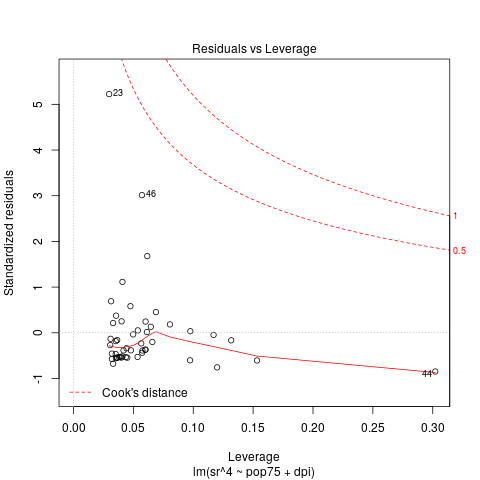
\includegraphics[scale=0.48]{imgR/plot25.png} \\
    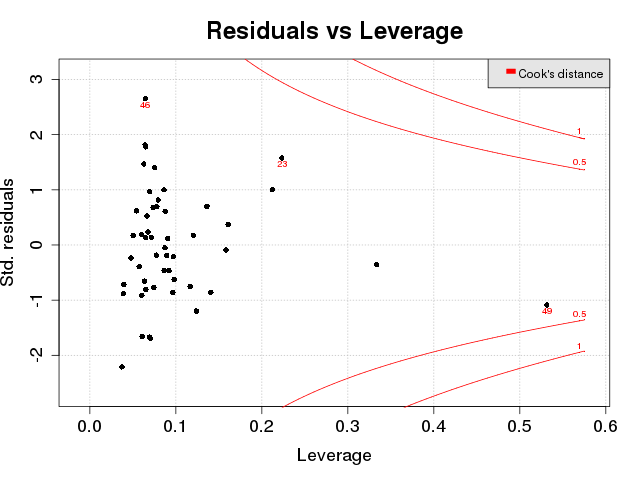
\includegraphics[scale=0.4]{imgOT/model1-drawResidualsVsLeverages.png}\hspace*{1cm}
	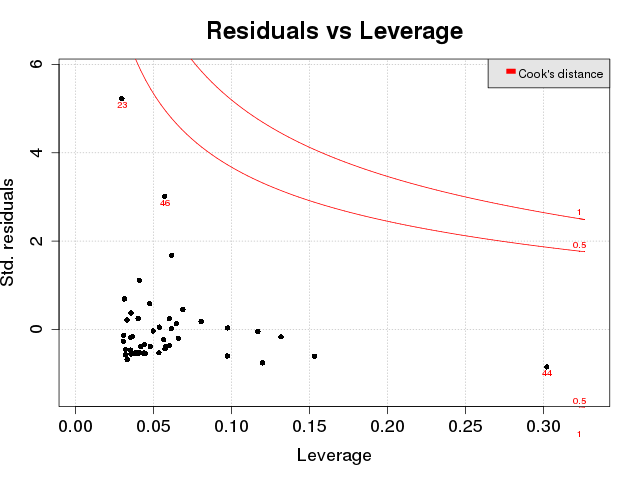
\includegraphics[scale=0.4]{imgOT/model2-drawResidualsVsLeverages.png}\\
  \end{center}
  \caption{Draw residuals versus leverages that adds bands corresponding to Cook's distances of 0.5 and 1. :\newline
  (Upper left: \textbf{\color{black}{model1: R output}}) (Upper right: \textbf{\color{black}{model2: R output}}) \newline
  (Lower left: \textbf{\color{blue}{model1: python output}})  (Lower right: \textbf{\color{blue}{model2: python output}}) }
\end{figure}

\begin{figure}[p]
  \begin{center}
    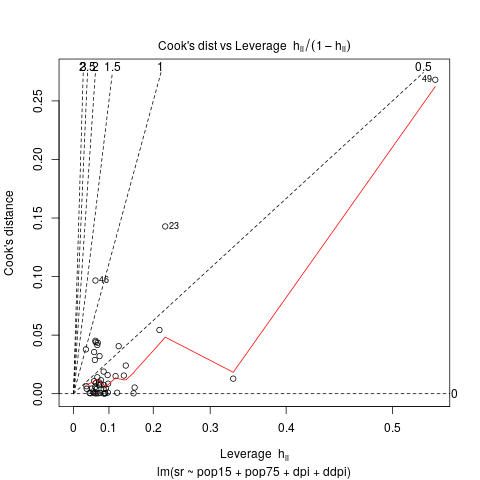
\includegraphics[scale=0.48]{imgR/plot16.png} \hspace*{2cm}
	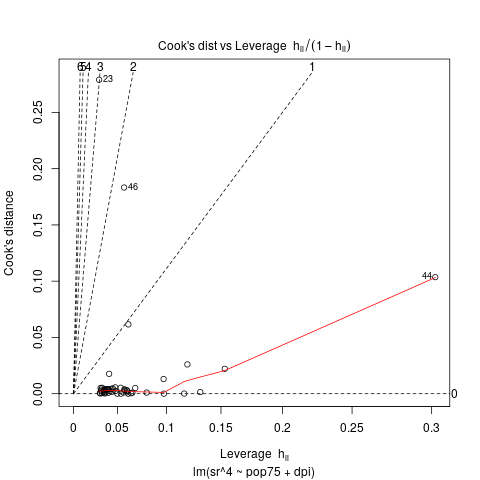
\includegraphics[scale=0.48]{imgR/plot26.png} \\
    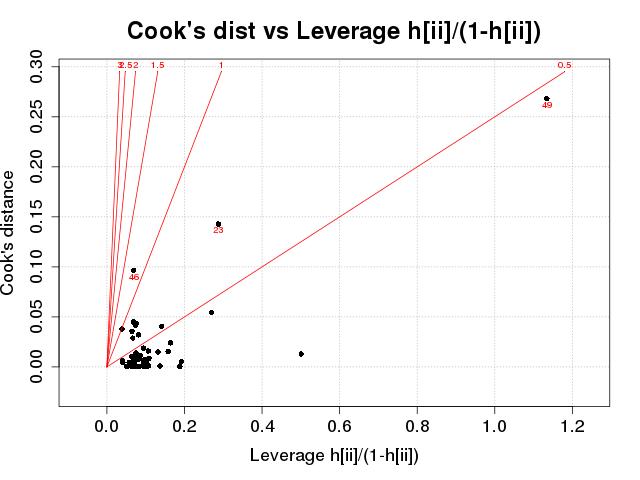
\includegraphics[scale=0.4]{imgOT/model1-drawCookVsLeverages.png}\hspace*{1cm}
	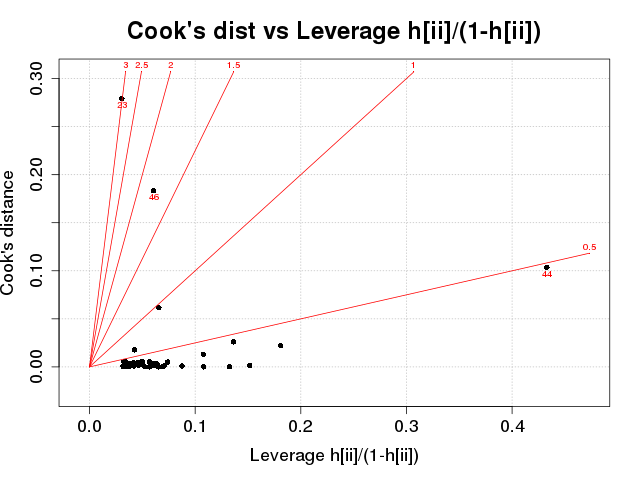
\includegraphics[scale=0.4]{imgOT/model2-drawCookVsLeverages.png}\\
  \end{center}
  \caption{Draw Cook's distances versus leverage/(1-leverage) : \newline
    (Upper left: \textbf{\color{black}{model1: R output}}) (Upper right: \textbf{\color{black}{model2: R output}}) \newline
  (Lower left: \textbf{\color{blue}{model1: python output}})  (Lower right: \textbf{\color{blue}{model2: python output}}) }
\end{figure}

\newpage
\subsection{Step method}

\subsubsection{Test1:}

R listing
\begin{lstlisting}[style=RStyle,basicstyle=\tiny]
### DESIGN
X <- data.frame(cbind(X1,X2,X3,X4))
names(X) <- c("X1","X2","X3","X4")

### LINEAR MODEL
myLinearModel <- function(X) {
    beta <- c (14 , -7 , -17 , -7 , -3 ,13 , -16 , -4 ,12 ,3 ,13 ,20 ,17 , -10 ,7)
    Design <- cbind(rep(1,dim(X)[1]),X[,1],X[,2],X[,3],X[,4], X[,3]^2,X[,4]^2,X[,1]^2,X[,1]*X[,2],
                       X[,2]*X[,4] , X[,3]*X[,4] , X[,1]*X[,2]*X[,3] , X[,1]^3 ,X[,2]^3 ,X[,4]^3 )
    Y <- Design%*%as.matrix(beta)
    return(Y)
}

### OBSERVATIONS
Y <- myLinearModel(X) + residuals

### MIN/MAX/START MODELS
model_min <- lm(Y~1 , data=X)
model_max <- lm(Y~(X1+X2+X3+X4)^3+I(X1^2)+I(X1^3)+I(X2^2)+I(X2^3)
                                 +I(X3^2)+I(X3^3)+I(X4^2)+I(X4^3), data=X)
model_0 <- lm(Y~X1+X2+X3+X4 , data=X)


### STEPWISE PROCEDURE

## Forward
#AIC
lm_forward_AIC <- step( model_min , scope=list(lower=model_min , upper=model_max) , direction="forward" , k=2)
#BIC
lm_forward_BIC <- step( model_min , scope=list(lower=model_min , upper=model_max) , direction="forward" , k=log(100))


## Backward
#AIC
lm_backward_AIC <- step( model_max , scope=list(lower=model_min , upper=model_max) , direction="backward" , k=2)
#BIC
lm_backward_BIC <- step( model_max , scope=list(upper=model_max , lower=model_min) , direction="backward" , k=log(100))

## Both
#AIC
lm_both_AIC <- step( model_0 , scope=list(lower=model_min , upper=model_max) , direction="both" , k=2)
#BIC
lm_both_BIC <- step( model_0 , scope=list(upper=model_max , lower=model_min) , direction="both" , k=log(100))


### ANOVA
summary(lm_forward_AIC)
summary(lm_backward_AIC)
summary(lm_both_AIC)

summary(lm_backward_BIC)
summary(lm_forward_BIC)
summary(lm_both_BIC)
\end{lstlisting}

Output
\begin{lstlisting}[style=output,basicstyle=\tiny]
> summary(lm_forward_AIC)

Call:
lm(formula = Y ~ I(X1^3) + I(X3^3) + I(X2^3) + X4 + X3 + I(X4^2) + 
    X4:X3, data = X)

Residuals:
    Min      1Q  Median      3Q     Max 
-4.8365 -1.3917 -0.1784  1.3654  6.4746 

Coefficients:
            Estimate Std. Error t value Pr(>|t|)    
(Intercept)   6.0459     1.1309   5.346 6.50e-07 ***
I(X1^3)      18.2477     0.8509  21.445  < 2e-16 ***
I(X3^3)      11.9240     1.9668   6.062 2.92e-08 ***
I(X2^3)     -16.6636     0.7983 -20.875  < 2e-16 ***
X4           -6.1208     3.6041  -1.698   0.0928 .  
X3           -0.2942     2.3979  -0.123   0.9026    
I(X4^2)      -7.6170     3.2805  -2.322   0.0224 *  
X4:X3        16.4005     2.9115   5.633 1.91e-07 ***
---
Signif. codes:  0 '***' 0.001 '**' 0.01 '*' 0.05 '.' 0.1 ' ' 1

Residual standard error: 2.193 on 92 degrees of freedom
Multiple R-squared:  0.9423,	Adjusted R-squared:  0.9379 
F-statistic: 214.5 on 7 and 92 DF,  p-value: < 2.2e-16
 
> summary(lm_backward_AIC)

Call:
lm(formula = Y ~ X1 + X2 + X3 + X4 + I(X1^3) + I(X2^3) + I(X3^2) + 
    I(X4^3) + X1:X2 + X1:X3 + X1:X4 + X2:X3 + X2:X4 + X3:X4 + 
    X1:X2:X3 + X2:X3:X4, data = X)

Residuals:
    Min      1Q  Median      3Q     Max 
-1.8223 -0.6065 -0.1239  0.5478  2.1709 

Coefficients:
            Estimate Std. Error t value Pr(>|t|)    
(Intercept)  14.8638     0.9518  15.617  < 2e-16 ***
X1           -5.7515     1.6671  -3.450 0.000884 ***
X2          -19.2572     1.9888  -9.683 2.82e-15 ***
X3           -9.6846     2.0988  -4.614 1.42e-05 ***
X4          -11.4020     1.6285  -7.001 6.07e-10 ***
I(X1^3)      14.5914     0.9685  15.065  < 2e-16 ***
I(X2^3)     -12.0528     0.9520 -12.660  < 2e-16 ***
I(X3^2)      13.9339     1.3449  10.361  < 2e-16 ***
I(X4^3)      -3.2383     0.9251  -3.500 0.000750 ***
X1:X2        11.4580     2.4410   4.694 1.05e-05 ***
X1:X3         1.8396     2.6413   0.696 0.488072    
X1:X4        -3.5140     1.3175  -2.667 0.009197 ** 
X2:X3         6.3360     3.2129   1.972 0.051936 .  
X2:X4        10.4012     2.7908   3.727 0.000353 ***
X3:X4        16.6128     2.4389   6.812 1.42e-09 ***
X1:X2:X3     14.5751     4.2878   3.399 0.001041 ** 
X2:X3:X4     -9.2093     4.2582  -2.163 0.033439 *  
---
Signif. codes:  0 '***' 0.001 '**' 0.01 '*' 0.05 '.' 0.1 ' ' 1

Residual standard error: 0.8908 on 83 degrees of freedom
Multiple R-squared:  0.9914,	Adjusted R-squared:  0.9897 
F-statistic: 598.4 on 16 and 83 DF,  p-value: < 2.2e-16


> summary(lm_both_AIC)

Call:
lm(formula = Y ~ X1 + X2 + X3 + X4 + I(X3^3) + I(X2^3) + I(X4^3) + 
    I(X1^3) + X1:X2 + X3:X4 + X1:X3 + X2:X3 + X2:X4 + X1:X4 + 
    X1:X2:X3 + X2:X3:X4, data = X)

Residuals:
    Min      1Q  Median      3Q     Max 
-1.8262 -0.5757 -0.1136  0.5819  2.1623 

Coefficients:
            Estimate Std. Error t value Pr(>|t|)    
(Intercept)  14.2255     0.9462  15.034  < 2e-16 ***
X1           -5.4113     1.6658  -3.249 0.001675 ** 
X2          -19.0700     1.9910  -9.578 4.56e-15 ***
X3           -3.8607     1.8558  -2.080 0.040572 *  
X4          -11.5169     1.6280  -7.074 4.38e-10 ***
I(X3^3)       9.1562     0.8829  10.370  < 2e-16 ***
I(X2^3)     -12.3189     0.9557 -12.890  < 2e-16 ***
I(X4^3)      -3.3016     0.9245  -3.571 0.000594 ***
I(X1^3)      14.3734     0.9717  14.792  < 2e-16 ***
X1:X2        11.0549     2.4375   4.535 1.92e-05 ***
X3:X4        17.1474     2.4374   7.035 5.22e-10 ***
X1:X3         0.8662     2.6440   0.328 0.744023    
X2:X3         6.6310     3.2090   2.066 0.041911 *  
X2:X4        10.5725     2.7884   3.792 0.000283 ***
X1:X4        -3.1422     1.3231  -2.375 0.019861 *  
X1:X2:X3     15.4381     4.2834   3.604 0.000533 ***
X2:X3:X4    -10.1590     4.2559  -2.387 0.019258 *  
---
Signif. codes:  0 '***' 0.001 '**' 0.01 '*' 0.05 '.' 0.1 ' ' 1

Residual standard error: 0.8904 on 83 degrees of freedom
Multiple R-squared:  0.9914,	Adjusted R-squared:  0.9898 
F-statistic:   599 on 16 and 83 DF,  p-value: < 2.2e-16
...
\end{lstlisting}

\newpage
Equivalent listing in python
\begin{lstlisting}[style=pythonStyle,basicstyle=\tiny]
import openturns as ot
from math import log

Sample = ot.NumericalSample.ImportFromTextFile("DATA_test1.csv", ",")

X = Sample[:, 1:5]
R = Sample[:, 0]

myLinearModel = ot.NumericalMathFunction(['x1', 'x2', 'x3', 'x4'], ['y'],
    ['14 - 7*x1 - 17*x2 - 7 *x3 - 3*x4 + 13*x3^2 - 16*x4^2 ' +
       ' - 4*x1^2 + 12*x1*x2 + 3*x2*x4 + 13*x3*x4 + 20*x1*x2*x3 ' +
       ' + 17*x1^3 - 10*x2^3 + 7*x4^3'])

Y = myLinearModel(X) + R

################################################################################################
# Build a model Y~(X1+X2+X3+X4)^3+I(Xi)^2+I(Xi)^3
dim = X.getDimension()
enumerateFunction = ot.EnumerateFunction(dim)
factory = ot.OrthogonalProductPolynomialFactory([ot.MonomialFactory()]*dim, enumerateFunction)

# Build 'interactions' as a list of list [a1,a2,a3,a4], and we will generate tensorized
# polynomials x1^a1*x2^a2*x3^a3*x4^a4.

# Y ~ (X1+X2+X3+X4)^4
interactions = [x for x in ot.Tuples([2]*dim).generate()]
# Remove X1*X2*X3*X4 to obtain Y ~ (X1+X2+X3+X4)^3
interactions.pop(interactions.index([1]*dim))
for i in xrange(dim):
  indices = [0]*dim
  indices[i] = 2
  # Y ~ I(Xi)^2
  interactions.append(indices[:])
  # Y ~ I(Xi)^3
  indices[i] = 3
  interactions.append(indices[:])

basis = ot.Basis([factory.build(enumerateFunction.inverse(indices)) for indices in interactions])
################################################################################################

i_min = [interactions.index([0,0,0,0])]
i_0 = i_min[:]
for i in xrange(dim):
  indices = [0]*dim
  indices[i] = 1
  i_0.append(interactions.index(indices))
i_0 = [i_0]

#---------------- Forward / Backward------------------- 
#   X: input sample
#   basis : Basis
#   Y: output sample
#   i_min:  indices of minimal model
#   direction: Boolean (True FORWARD, False BACKWARD)
#   penalty: multiplier of number of degrees of freedom
#   maxiteration: maximum number of iterations

#---------------- Both------------------- 
#   X: input sample
#   basis : Basis
#   Y: output sample
#   i_min : indices of minimal model
#   i_0   : indices of start model
#   penalty: multiplier of number of degrees of freedom
#   maxiteration: maximum number of iterations

penalty_BIC = log(X.getSize())
penalty_AIC = 2.
maxiteration = 1000

for k in [penalty_AIC, penalty_BIC]:
  ## Forward / Backward
  if k==penalty_AIC:  IC =" AIC "
  if k==penalty_BIC:  IC =" BIC "  
  for forward in [True, False]:
    algo = ot.LinearModelStepwiseAlgorithm(X, basis, Y, i_min, forward, k, maxiteration)
    algo_result = ot.LinearModelAnalysis(algo.getResult())
    print("{0:~^60s}".format(""))
    if forward==True : print(" Forward " +IC)
    else             : print(" Backward "+IC)
    print("{0:~^60s}".format(""))
    print(algo_result)
  ## Both
  algo = ot.LinearModelStepwiseAlgorithm(X, basis, Y, i_min, i_0, k, maxiteration)
  algo_result = ot.LinearModelAnalysis(algo.getResult())
  print("{0:~^60s}".format(""))
  print(" Both "+IC)
  print("{0:~^60s}".format(""))
  print(algo_result)
\end{lstlisting}

\newpage
Output python
\begin{lstlisting}[style=output,basicstyle=\tiny]
~~~~~~~~~~~~~~~~~~~~~~~~~~~~~~~~~~~~~~~~~~~~~~~~~~~~~~~~~~~~
 Forward  AIC 
~~~~~~~~~~~~~~~~~~~~~~~~~~~~~~~~~~~~~~~~~~~~~~~~~~~~~~~~~~~~

 Call:
Basis( [1,x0,x1,(x0) * (x1),x2,(x0) * (x2),(x1) * (x2),(x0) * (x1) * (x2),x3,(x0) * (x3),(x1) * (x3),(x0) * (x1) * (x3),(x2) * (x3),(x0) * (x2) * (x3),(x1) * (x2) * (x3),x0^2,x0^3,x1^2,x1^3,x2^2,x2^3,x3^2,x3^3]#23 )

 Coefficients:
                   | Estimate    | Std Error   | t value     | Pr(>|t|)    | 
----------------------------------------------------------------------------
1                  | 10.9814     | 0.65648     | 16.7277     | 1.27112e-28 | 
x1                 | -3.88875    | 1.9846      | -1.95946    | 0.0533367   | 
(x0) * (x1)        | 7.18917     | 8.49215     | 0.846566    | 0.399614    | 
(x0) * (x2)        | 18.6503     | 2.15953     | 8.63624     | 2.94296e-13 | 
(x0) * (x1) * (x2) | 9.55935     | 0.861055    | 11.1019     | 3.21154e-18 | 
x3                 | 14.3043     | 1.03648     | 13.8009     | 2.04805e-23 | 
(x0) * (x3)        | -11.6087    | 1.83235     | -6.33539    | 1.08208e-08 | 
(x0) * (x1) * (x3) | 9.8174      | 2.11831     | 4.63455     | 1.28003e-05 | 
(x2) * (x3)        | 5.86969     | 2.9541      | 1.98696     | 0.0501475   | 
(x0) * (x2) * (x3) | -4.64921    | 1.50572     | -3.0877     | 0.00272418  | 
x0^3               | 9.9525      | 1.56499     | 6.35948     | 9.73106e-09 | 
x1^2               | -16.4775    | 3.73193     | -4.41527    | 2.94963e-05 | 
x1^3               | -16.4804    | 5.66605     | -2.90862    | 0.00463118  | 
x2^3               | 4.14884     | 1.9234      | 2.15704     | 0.033826    | 
x3^2               | -3.25933    | 1.65126     | -1.97385    | 0.0516471   | 
----------------------------------------------------------------------------

 Residual standard error: 0.93463 on 85 degrees of freedom 
 F-statistic: 620.59 ,  p-value: 0
---------------------------------
Multiple R-squared   | 0.990312 | 
Adjusted R-squared   | 0.988716 | 
---------------------------------

---------------------------------
Normality test       | p-value  | 
---------------------------------
Anderson-Darling     | 0.132184 | 
Chi-Squared          | 0.562718 | 
Kolmogorov-Smirnov   | 0.620456 | 
---------------------------------

~~~~~~~~~~~~~~~~~~~~~~~~~~~~~~~~~~~~~~~~~~~~~~~~~~~~~~~~~~~~
 Backward  AIC 
~~~~~~~~~~~~~~~~~~~~~~~~~~~~~~~~~~~~~~~~~~~~~~~~~~~~~~~~~~~~

 Call:
Basis( [1,x0,x1,(x0) * (x1),x2,(x0) * (x2),(x1) * (x2),(x0) * (x1) * (x2),x3,(x0) * (x3),(x1) * (x3),(x0) * (x1) * (x3),(x2) * (x3),(x0) * (x2) * (x3),(x1) * (x2) * (x3),x0^2,x0^3,x1^2,x1^3,x2^2,x2^3,x3^2,x3^3]#23 )

 Coefficients:
                   | Estimate    | Std Error   | t value     | Pr(>|t|)    | 
----------------------------------------------------------------------------
1                  | 14.4696     | 0.85367     | 16.9499     | 1.10055e-28 | 
x0                 | -4.96924    | 1.13775     | -4.36761    | 3.6037e-05  | 
x1                 | -19.6298    | 1.96072     | -10.0115    | 6.24137e-16 | 
(x0) * (x1)        | 11.8902     | 2.08797     | 5.6946      | 1.82096e-07 | 
x2                 | -8.79793    | 1.85144     | -4.75195    | 8.3525e-06  | 
(x1) * (x2)        | 6.52733     | 2.99453     | 2.17975     | 0.0321087   | 
(x0) * (x1) * (x2) | 13.9549     | 3.1442      | 4.43829     | 2.76759e-05 | 
x3                 | -10.1758    | 1.96078     | -5.18967    | 1.46874e-06 | 
(x0) * (x3)        | -5.60052    | 2.132       | -2.62688    | 0.0102606   | 
(x1) * (x3)        | 10.2331     | 2.74482     | 3.72817     | 0.000351322 | 
(x2) * (x3)        | 14.3123     | 3.13008     | 4.57249     | 1.66633e-05 | 
(x0) * (x2) * (x3) | 3.92134     | 3.01451     | 1.30082     | 0.19692     | 
(x1) * (x2) * (x3) | -8.77332    | 4.2304      | -2.07388    | 0.0411906   | 
x0^3               | 14.768      | 0.974922    | 15.1479     | 1.30072e-25 | 
x1^3               | -11.8816    | 0.958026    | -12.4021    | 1.36769e-20 | 
x2^2               | 14.0536     | 1.33682     | 10.5127     | 6.33754e-17 | 
x3^3               | -3.25468    | 0.917225    | -3.54839    | 0.000640898 | 
----------------------------------------------------------------------------

 Residual standard error: 0.88446 on 83 degrees of freedom 
 F-statistic: 607.11 ,  p-value: 0
---------------------------------
Multiple R-squared   | 0.991528 | 
Adjusted R-squared   | 0.989895 | 
---------------------------------

---------------------------------
Normality test       | p-value  | 
---------------------------------
Anderson-Darling     | 0.197651 | 
Chi-Squared          | 0.125636 | 
Kolmogorov-Smirnov   | 0.482042 | 
---------------------------------

~~~~~~~~~~~~~~~~~~~~~~~~~~~~~~~~~~~~~~~~~~~~~~~~~~~~~~~~~~~~
 Both  AIC 
~~~~~~~~~~~~~~~~~~~~~~~~~~~~~~~~~~~~~~~~~~~~~~~~~~~~~~~~~~~~

 Call:
Basis( [1,x0,x1,(x0) * (x1),x2,(x0) * (x2),(x1) * (x2),(x0) * (x1) * (x2),x3,(x0) * (x3),(x1) * (x3),(x0) * (x1) * (x3),(x2) * (x3),(x0) * (x2) * (x3),(x1) * (x2) * (x3),x0^2,x0^3,x1^2,x1^3,x2^2,x2^3,x3^2,x3^3]#23 )

 Coefficients:
                   | Estimate    | Std Error   | t value     | Pr(>|t|)    | 
----------------------------------------------------------------------------
1                  | 10.9814     | 0.65648     | 16.7277     | 1.27112e-28 | 
x1                 | -3.88875    | 1.9846      | -1.95946    | 0.0533367   | 
(x0) * (x1)        | 7.18917     | 8.49215     | 0.846566    | 0.399614    | 
(x0) * (x2)        | 18.6503     | 2.15953     | 8.63624     | 2.94296e-13 | 
(x0) * (x1) * (x2) | 9.55935     | 0.861055    | 11.1019     | 3.21154e-18 | 
x3                 | 14.3043     | 1.03648     | 13.8009     | 2.04805e-23 | 
(x0) * (x3)        | -11.6087    | 1.83235     | -6.33539    | 1.08208e-08 | 
(x0) * (x1) * (x3) | 9.8174      | 2.11831     | 4.63455     | 1.28003e-05 | 
(x2) * (x3)        | 5.86969     | 2.9541      | 1.98696     | 0.0501475   | 
(x0) * (x2) * (x3) | -4.64921    | 1.50572     | -3.0877     | 0.00272418  | 
x0^3               | 9.9525      | 1.56499     | 6.35948     | 9.73106e-09 | 
x1^2               | -16.4775    | 3.73193     | -4.41527    | 2.94963e-05 | 
x1^3               | -16.4804    | 5.66605     | -2.90862    | 0.00463118  | 
x2^3               | 4.14884     | 1.9234      | 2.15704     | 0.033826    | 
x3^2               | -3.25933    | 1.65126     | -1.97385    | 0.0516471   | 
----------------------------------------------------------------------------

 Residual standard error: 0.93463 on 85 degrees of freedom 
 F-statistic: 620.59 ,  p-value: 0
---------------------------------
Multiple R-squared   | 0.990312 | 
Adjusted R-squared   | 0.988716 | 
---------------------------------

---------------------------------
Normality test       | p-value  | 
---------------------------------
Anderson-Darling     | 0.132184 | 
Chi-Squared          | 0.562718 | 
Kolmogorov-Smirnov   | 0.620456 | 
---------------------------------
...
\end{lstlisting}

\newpage
\subsubsection{Test2:}

R listing
\begin{lstlisting}[style=RStyle,basicstyle=\tiny]
### MIN/MAX MODELS
model_min <- lm( BIO~ 1 , data=DATA)
model_max <- lm( BIO~SAL+pH+K+Na+Zn , data=DATA)


### STEPWISE PROCEDURE
## Forward
model_0 <- lm( BIO~ 1 , data=DATA)
#AIC
lm_forward_AIC <- step( model_min , scope=list(lower=model_min , upper=model_max) , direction="forward" , k=2)
#BIC
lm_forward_BIC <- step( model_min , scope=list(lower=model_min , upper=model_max) , direction="forward" , k=log(45))

## Backward
model_0 <- lm( BIO~SAL+pH+K+Na+Zn , data=DATA)
#AIC
lm_backward_AIC <- step( model_max , scope=list( lower=model_min , upper=model_max) , direction="backward" , k=2)
#BIC
lm_backward_BIC <- step( model_max , scope=list( upper=model_max , lower=model_min) , direction="backward" , k=log(45))
## Both
model_0 <- lm( BIO~ 1 , data=DATA)
#AIC
lm_both_AIC <- step( model_0 , scope=list( lower=model_min , upper=model_max) , direction="both" , k=2)
#BIC
lm_both_BIC <- step( model_0 , scope=list( upper=model_max , lower=model_min) , direction="both" , k=log (45))


### ANOVA

summary(lm_forward_AIC)
summary(lm_backward_AIC)
summary(lm_both_AIC)

summary(lm_forward_BIC)
summary(lm_backward_BIC)
summary(lm_both_BIC)
\end{lstlisting}

\newpage
Output
\begin{lstlisting}[style=output,basicstyle=\tiny]
> summary(lm_forward_AIC)

Call:
lm(formula = BIO ~ pH + Na, data = DATA)

Residuals:
    Min      1Q  Median      3Q     Max 
-677.93 -229.76  -97.47  207.51 1168.40 

Coefficients:
              Estimate Std. Error t value Pr(>|t|)    
(Intercept) -4.757e+02  2.735e+02  -1.739   0.0893 .  
pH           4.049e+02  4.777e+01   8.477 1.22e-10 ***
Na          -2.333e-02  8.655e-03  -2.695   0.0101 *  
---
Signif. codes:  0 '***' 0.001 '**' 0.01 '*' 0.05 '.' 0.1 ' ' 1

Residual standard error: 394.9 on 42 degrees of freedom
Multiple R-squared:  0.6584,	Adjusted R-squared:  0.6422 
F-statistic: 40.48 on 2 and 42 DF,  p-value: 1.596e-10

> summary(lm_backward_AIC)

Call:
lm(formula = BIO ~ SAL + pH + K + Zn, data = DATA)

Residuals:
   Min     1Q Median     3Q    Max 
-749.1 -229.2  -94.2  127.2 1037.4 

Coefficients:
             Estimate Std. Error t value Pr(>|t|)   
(Intercept) 1505.4882  1133.6940   1.328  0.19172   
SAL          -35.9433    21.4761  -1.674  0.10201   
pH           293.8611    84.4738   3.479  0.00123 **
K             -0.4388     0.2024  -2.168  0.03615 * 
Zn           -23.4519    14.0399  -1.670  0.10265   
---
Signif. codes:  0 '***' 0.001 '**' 0.01 '*' 0.05 '.' 0.1 ' ' 1

Residual standard error: 394.8 on 40 degrees of freedom
Multiple R-squared:  0.6749,	Adjusted R-squared:  0.6423 
F-statistic: 20.76 on 4 and 40 DF,  p-value: 2.528e-09


> summary(lm_both_AIC)

Call:
lm(formula = BIO ~ pH + Na, data = DATA)

Residuals:
    Min      1Q  Median      3Q     Max 
-677.93 -229.76  -97.47  207.51 1168.40 

Coefficients:
              Estimate Std. Error t value Pr(>|t|)    
(Intercept) -4.757e+02  2.735e+02  -1.739   0.0893 .  
pH           4.049e+02  4.777e+01   8.477 1.22e-10 ***
Na          -2.333e-02  8.655e-03  -2.695   0.0101 *  
---
Signif. codes:  0 '***' 0.001 '**' 0.01 '*' 0.05 '.' 0.1 ' ' 1

Residual standard error: 394.9 on 42 degrees of freedom
Multiple R-squared:  0.6584,	Adjusted R-squared:  0.6422 
F-statistic: 40.48 on 2 and 42 DF,  p-value: 1.596e-10

...
\end{lstlisting}

\newpage
Equivalent listing in python
\begin{lstlisting}[style=pythonStyle,basicstyle=\tiny]
import openturns as ot
from math import log

Sample = ot.NumericalSample.ImportFromTextFile("DATA_test2.csv", ",")
# Sample.setDescription(["BIO","SAL","pH","K","Na","Zn"])
print(Sample)

X = Sample[:, 1:6]
Y = Sample[:, 0]

################################################################################################
# Build a model BIO~SAL+pH+K+Na+Zn
dim = X.getDimension()
enumerateFunction = ot.EnumerateFunction(dim)
factory = ot.OrthogonalProductPolynomialFactory([ot.MonomialFactory()]*dim, enumerateFunction)

# Build 'interactions' as a list of list [a1,a2,a3,a4,a5], and we will generate tensorized
# polynomials SAL^a1*pH^a2*K^a3*Na^a4*Zn^a5.

# BIO~SAL+pH+K+Na+Zn
interactions = []
interactions.append([0]*dim)
for i in xrange(dim):
  indices = [0]*dim
  indices[i] = 1
  # Y ~ I(Xi)^1
  interactions.append(indices[:])

basis = ot.Basis([factory.build(enumerateFunction.inverse(indices)) for indices in interactions])
################################################################################################

i_min = [interactions.index([0,0,0,0,0])]
i_0 = i_min[:]

#---------------- Forward / Backward------------------- 
#   X: input sample
#   basis : Basis
#   Y: output sample
#   i_min:  indices of minimal model
#   direction: Boolean (True FORWARD, False BACKWARD)
#   penalty: multiplier of number of degrees of freedom
#   maxiteration: maximum number of iterations

#---------------- Both------------------- 
#   X: input sample
#   basis : Basis
#   Y: output sample
#   i_min : indices of minimal model
#   i_0   : indices of start model
#   penalty: multiplier of number of degrees of freedom
#   maxiteration: maximum number of iterations

penalty_BIC = log(X.getSize())
penalty_AIC = 2.
maxiteration = 1000

for k in [penalty_AIC, penalty_BIC]:
  ## Forward / Backward
  if k==penalty_AIC:  IC =" AIC "
  if k==penalty_BIC:  IC =" BIC "  
  for forward in [True, False]:
    algo = ot.LinearModelStepwiseAlgorithm(X, basis, Y, i_min, forward, k, maxiteration)
    algo_result = ot.LinearModelAnalysis(algo.getResult())
    print("{0:~^60s}".format(""))
    if forward==True : print(" Forward " +IC)
    else             : print(" Backward "+IC)
    print("{0:~^60s}".format(""))
    print(algo_result)
  ## Both
  algo = ot.LinearModelStepwiseAlgorithm(X, basis, Y, i_min, i_0, k, maxiteration)
  algo_result = ot.LinearModelAnalysis(algo.getResult())
  print("{0:~^60s}".format(""))
  print(" Both "+IC)
  print("{0:~^60s}".format(""))
  print(algo_result)
\end{lstlisting}

\newpage
Output python
\begin{lstlisting}[style=output,basicstyle=\tiny]
~~~~~~~~~~~~~~~~~~~~~~~~~~~~~~~~~~~~~~~~~~~~~~~~~~~~~~~~~~~~
 Forward  AIC 
~~~~~~~~~~~~~~~~~~~~~~~~~~~~~~~~~~~~~~~~~~~~~~~~~~~~~~~~~~~~
 Call:
Basis( [1,x0,x1,x2,x3,x4] )

 Coefficients:
   | Estimate    | Std Error   | t value     | Pr(>|t|)    | 
------------------------------------------------------------
1  | -475.729    | 273.522     | -1.73927    | 0.0893122   | 
x1 | 404.948     | 47.7698     | 8.47707     | 1.22026e-10 | 
x3 | -0.0233259  | 0.00865512  | -2.69504    | 0.0100775   | 
------------------------------------------------------------

 Residual standard error: 394.85 on 42 degrees of freedom 
 F-statistic: 40.481 ,  p-value: 1.0636e-10
---------------------------------
Multiple R-squared   | 0.658433 | 
Adjusted R-squared   | 0.642168 | 
---------------------------------

------------------------------------
Normality test       | p-value     | 
------------------------------------
Anderson-Darling     | 0.000429122 | 
Chi-Squared          | 0.000909433 | 
Kolmogorov-Smirnov   | 0.0481525   | 
------------------------------------

~~~~~~~~~~~~~~~~~~~~~~~~~~~~~~~~~~~~~~~~~~~~~~~~~~~~~~~~~~~~
 Backward  AIC 
~~~~~~~~~~~~~~~~~~~~~~~~~~~~~~~~~~~~~~~~~~~~~~~~~~~~~~~~~~~~
 Call:
Basis( [1,x0,x1,x2,x3,x4] )

 Coefficients:
   | Estimate   | Std Error  | t value    | Pr(>|t|)   | 
--------------------------------------------------------
1  | 1505.49    | 1133.69    | 1.32795    | 0.191723   | 
x0 | -35.9433   | 21.4761    | -1.67364   | 0.102005   | 
x1 | 293.861    | 84.4738    | 3.47873    | 0.00123036 | 
x2 | -0.438818  | 0.202384   | -2.16824   | 0.0361463  | 
x4 | -23.4519   | 14.0399    | -1.67038   | 0.102653   | 
--------------------------------------------------------

 Residual standard error: 394.76 on 40 degrees of freedom 
 F-statistic: 20.756 ,  p-value: 1.1414e-09
---------------------------------
Multiple R-squared   | 0.674859 | 
Adjusted R-squared   | 0.642344 | 
---------------------------------

-----------------------------------
Normality test       | p-value    | 
-----------------------------------
Anderson-Darling     | 0.00124009 | 
Chi-Squared          | 0.0204981  | 
Kolmogorov-Smirnov   | 0.338063   | 
-----------------------------------

~~~~~~~~~~~~~~~~~~~~~~~~~~~~~~~~~~~~~~~~~~~~~~~~~~~~~~~~~~~~
 Both  AIC 
~~~~~~~~~~~~~~~~~~~~~~~~~~~~~~~~~~~~~~~~~~~~~~~~~~~~~~~~~~~~
 Call:
Basis( [1,x0,x1,x2,x3,x4] )

 Coefficients:
   | Estimate    | Std Error   | t value     | Pr(>|t|)    | 
------------------------------------------------------------
1  | -475.729    | 273.522     | -1.73927    | 0.0893122   | 
x1 | 404.948     | 47.7698     | 8.47707     | 1.22026e-10 | 
x3 | -0.0233259  | 0.00865512  | -2.69504    | 0.0100775   | 
------------------------------------------------------------

 Residual standard error: 394.85 on 42 degrees of freedom 
 F-statistic: 40.481 ,  p-value: 1.0636e-10
---------------------------------
Multiple R-squared   | 0.658433 | 
Adjusted R-squared   | 0.642168 | 
---------------------------------

------------------------------------
Normality test       | p-value     | 
------------------------------------
Anderson-Darling     | 0.000429122 | 
Chi-Squared          | 0.000909433 | 
Kolmogorov-Smirnov   | 0.0481525   | 
------------------------------------
...
\end{lstlisting}



